\documentclass[tikz,border=12pt]{standalone}
\usepackage[svgnames]{xcolor}
\usepackage{tikz}
\usetikzlibrary{arrows.meta,calc,positioning}

\begin{document}
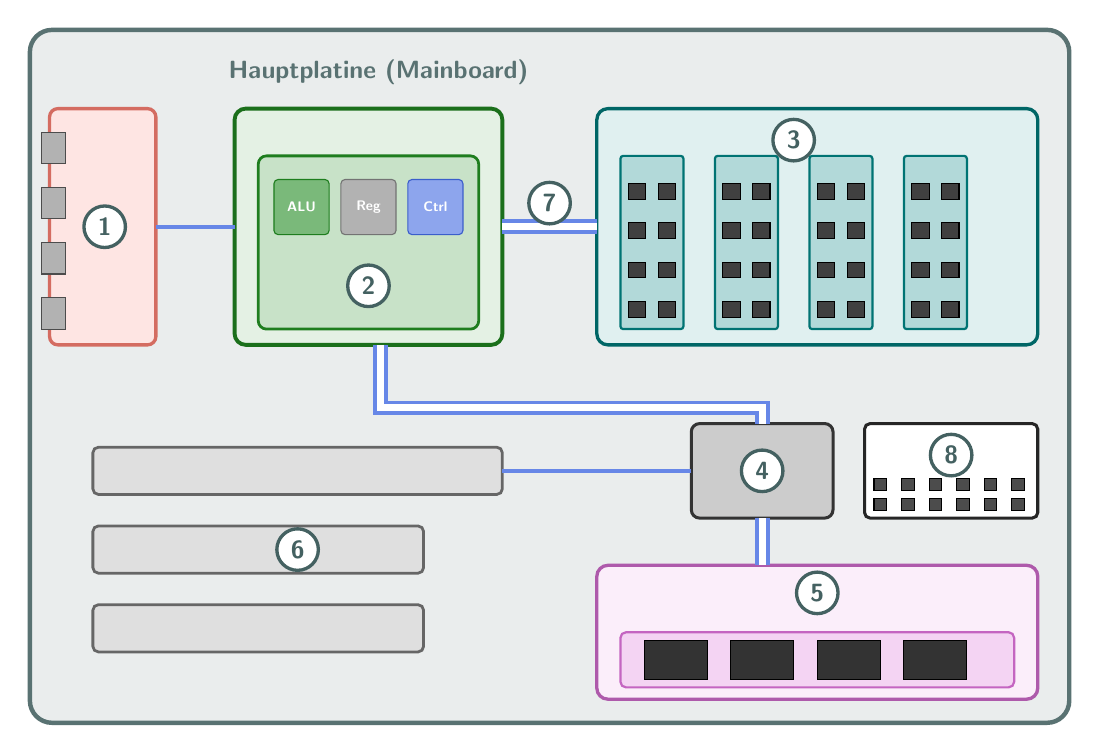
\begin{tikzpicture}[
    scale=1.0,
    every node/.style={transform shape},
    board/.style={fill=DarkSlateGray!10, draw=DarkSlateGray!80, line width=1.6pt, rounded corners=8pt},
    trace/.style={draw=RoyalBlue!80, line width=1.4pt},
    badge/.style={circle, draw=DarkSlateGray!90, fill=white, line width=1.2pt, inner sep=2.5pt, font=\bfseries\sffamily\small, text=DarkSlateGray!90}
]
    % --- Mainboard Platine ---
    \draw[board] (-6.6, -4.4) rectangle (6.6, 4.4);
    \node[anchor=north west, font=\bfseries\sffamily\small, text=DarkSlateGray!80] at (-4.2, 4.15) {Hauptplatine (Mainboard)};

    % --- 1. I/O-Panel (links) ---
    \draw[fill=Salmon!20, draw=Salmon!85!black, line width=1.2pt, rounded corners=3pt] (-6.35, 0.4) rectangle (-5.0, 3.4);
    \foreach \y in {0.8, 1.5, 2.2, 2.9} {
        \draw[fill=gray!60, draw=black!70] (-6.45, \y-0.2) rectangle (-6.15, \y+0.2);
    }
    \node[badge] at (-5.65, 1.9) {1};

    % --- 2. CPU-Sockel & Prozessor (Mitte-Links) ---
    \draw[fill=ForestGreen!12, draw=ForestGreen!80!black, line width=1.4pt, rounded corners=4pt] (-4.0, 0.4) rectangle (-0.6, 3.4);
    \draw[fill=ForestGreen!25, draw=ForestGreen!90!black, line width=1pt, rounded corners=3pt] (-3.7, 0.6) rectangle (-0.9, 2.8);
    % Sub-blocks (ALU, Reg, Steuerwerk)
    \draw[fill=ForestGreen!60, draw=ForestGreen!90!black, rounded corners=1.5pt] (-3.5, 1.8) rectangle (-2.8, 2.5);
    \node[font=\tiny\bfseries\sffamily, text=white] at (-3.15, 2.15) {ALU};
    
    \draw[fill=Gray!60, draw=Gray!90!black, rounded corners=1.5pt] (-2.65, 1.8) rectangle (-1.95, 2.5);
    \node[font=\tiny\bfseries\sffamily, text=white] at (-2.3, 2.15) {Reg};
    
    \draw[fill=RoyalBlue!60, draw=RoyalBlue!90!black, rounded corners=1.5pt] (-1.8, 1.8) rectangle (-1.1, 2.5);
    \node[font=\tiny\bfseries\sffamily, text=white] at (-1.45, 2.15) {Ctrl};
    
    \node[badge] at (-2.3, 1.15) {2};

    % --- 3. RAM-Bänke (Rechts oben) ---
    \draw[fill=Teal!12, draw=Teal!80!black, line width=1.2pt, rounded corners=4pt] (0.6, 0.4) rectangle (6.2, 3.4);
    % 4 RAM Riegel (DIMMs)
    \foreach \x in {1.3, 2.5, 3.7, 4.9} {
        \draw[fill=Teal!30, draw=Teal!90!black, line width=0.8pt, rounded corners=1pt] (\x-0.4, 0.6) rectangle (\x+0.4, 2.8);
        \foreach \y in {0.85, 1.35, 1.85, 2.35} {
            \draw[fill=black!75] (\x-0.3, \y-0.1) rectangle (\x-0.08, \y+0.1);
            \draw[fill=black!75] (\x+0.08, \y-0.1) rectangle (\x+0.3, \y+0.1);
        }
    }
    \node[badge] at (3.1, 3.0) {3};

    % --- 4. Chipsatz / Southbridge (Mitte) ---
    \draw[fill=gray!40, draw=black!80, line width=1.1pt, rounded corners=3pt] (1.8, -1.8) rectangle (3.6, -0.6);
    \node[badge] at (2.7, -1.2) {4};

    % --- 8. 24-Pin ATX Stromanschluss (Netzteil / PSU) (Mitte-Rechts) ---
    \draw[fill=white, draw=black!85, line width=1.1pt, rounded corners=2pt] (4.0, -1.8) rectangle (6.2, -0.6);
    \foreach \px in {4.2, 4.55, 4.9, 5.25, 5.6, 5.95} {
        \draw[fill=black!70] (\px-0.08, -1.45) rectangle (\px+0.08, -1.3);
        \draw[fill=black!70] (\px-0.08, -1.7) rectangle (\px+0.08, -1.55);
    }
    \node[badge] at (5.1, -1.0) {8};

    % --- 5. Massenspeicher (M.2 NVMe SSD Slot) (Rechts unten) ---
    \draw[fill=Orchid!12, draw=Orchid!80!black, line width=1.2pt, rounded corners=4pt] (0.6, -4.1) rectangle (6.2, -2.4);
    \draw[fill=Orchid!30, draw=Orchid!90!black, line width=0.8pt, rounded corners=2pt] (0.9, -3.95) rectangle (5.9, -3.25);
    \foreach \cx in {1.6, 2.7, 3.8, 4.9} {
        \draw[fill=black!80] (\cx-0.4, -3.85) rectangle (\cx+0.4, -3.35);
    }
    \node[badge] at (3.4, -2.75) {5};

    % --- 6. PCIe Steckplätze (Links unten) ---
    \draw[fill=gray!25, draw=black!60, line width=1pt, rounded corners=2pt] (-5.8, -1.5) rectangle (-0.6, -0.9);
    \draw[fill=gray!25, draw=black!60, line width=1pt, rounded corners=2pt] (-5.8, -2.5) rectangle (-1.6, -1.9);
    \draw[fill=gray!25, draw=black!60, line width=1pt, rounded corners=2pt] (-5.8, -3.5) rectangle (-1.6, -2.9);
    \node[badge] at (-3.2, -2.2) {6};

    % --- 7. Systembus & Speicherbus (Leiterbahnen) ---
    % CPU <-> RAM (Speicherbus)
    \draw[trace, double distance=2.5pt] (-0.6, 1.9) -- (0.6, 1.9);
    \node[badge] at (0.0, 2.2) {7};

    % CPU <-> I/O Panel
    \draw[trace] (-4.0, 1.9) -- (-5.0, 1.9);

    % CPU <-> Chipsatz
    \draw[trace, double distance=2.5pt] (-2.15, 0.4) -- (-2.15, -0.4) -- (2.7, -0.4) -- (2.7, -0.6);
    
    % Chipsatz <-> M.2 SSD
    \draw[trace, double distance=2.5pt] (2.7, -1.8) -- (2.7, -2.4);

    % Chipsatz <-> PCIe Slots
    \draw[trace] (1.8, -1.2) -- (-0.6, -1.2);

\end{tikzpicture}
\end{document}
